
\section{Silicon tracker}
\label{ss:cms_tracker}
Due to the small band gap (1.12\unit{eV}), high carrier mobility (1450 \unit{$\rm{cm}^2/Vs$}), 
and high specific density (2.33 \unit{$\rm{g}/\rm{cm}^3$}) the silicon detectors are used in 
the CMS experiment for the measurements of trajectory and momentum of the particles 
produced in the collision.
The silicon tracker of the CMS is closest to the beam axis. Its location is shown in 
Figure~\ref{fig:cms_tracker}. It has 3 (2) layers of pixel tracker in the barrel (endcap) region, and
10 (9) layers of the strip tracker in the barrel (endcap) region. There are about 48 
(18) million pixels in the barrel (endcap) region covering an area of 200\unit{$\rm{m}^2$} which
makes it the biggest silicon detector ever built in the world.
\begin{figure}
  \centering
  \subfigure[The inner part of one of the tracker inner barrels (TIBs) of the
	CMS experiment \cite{cmsInfo}.
  \label{subfig:cms_track}]
  {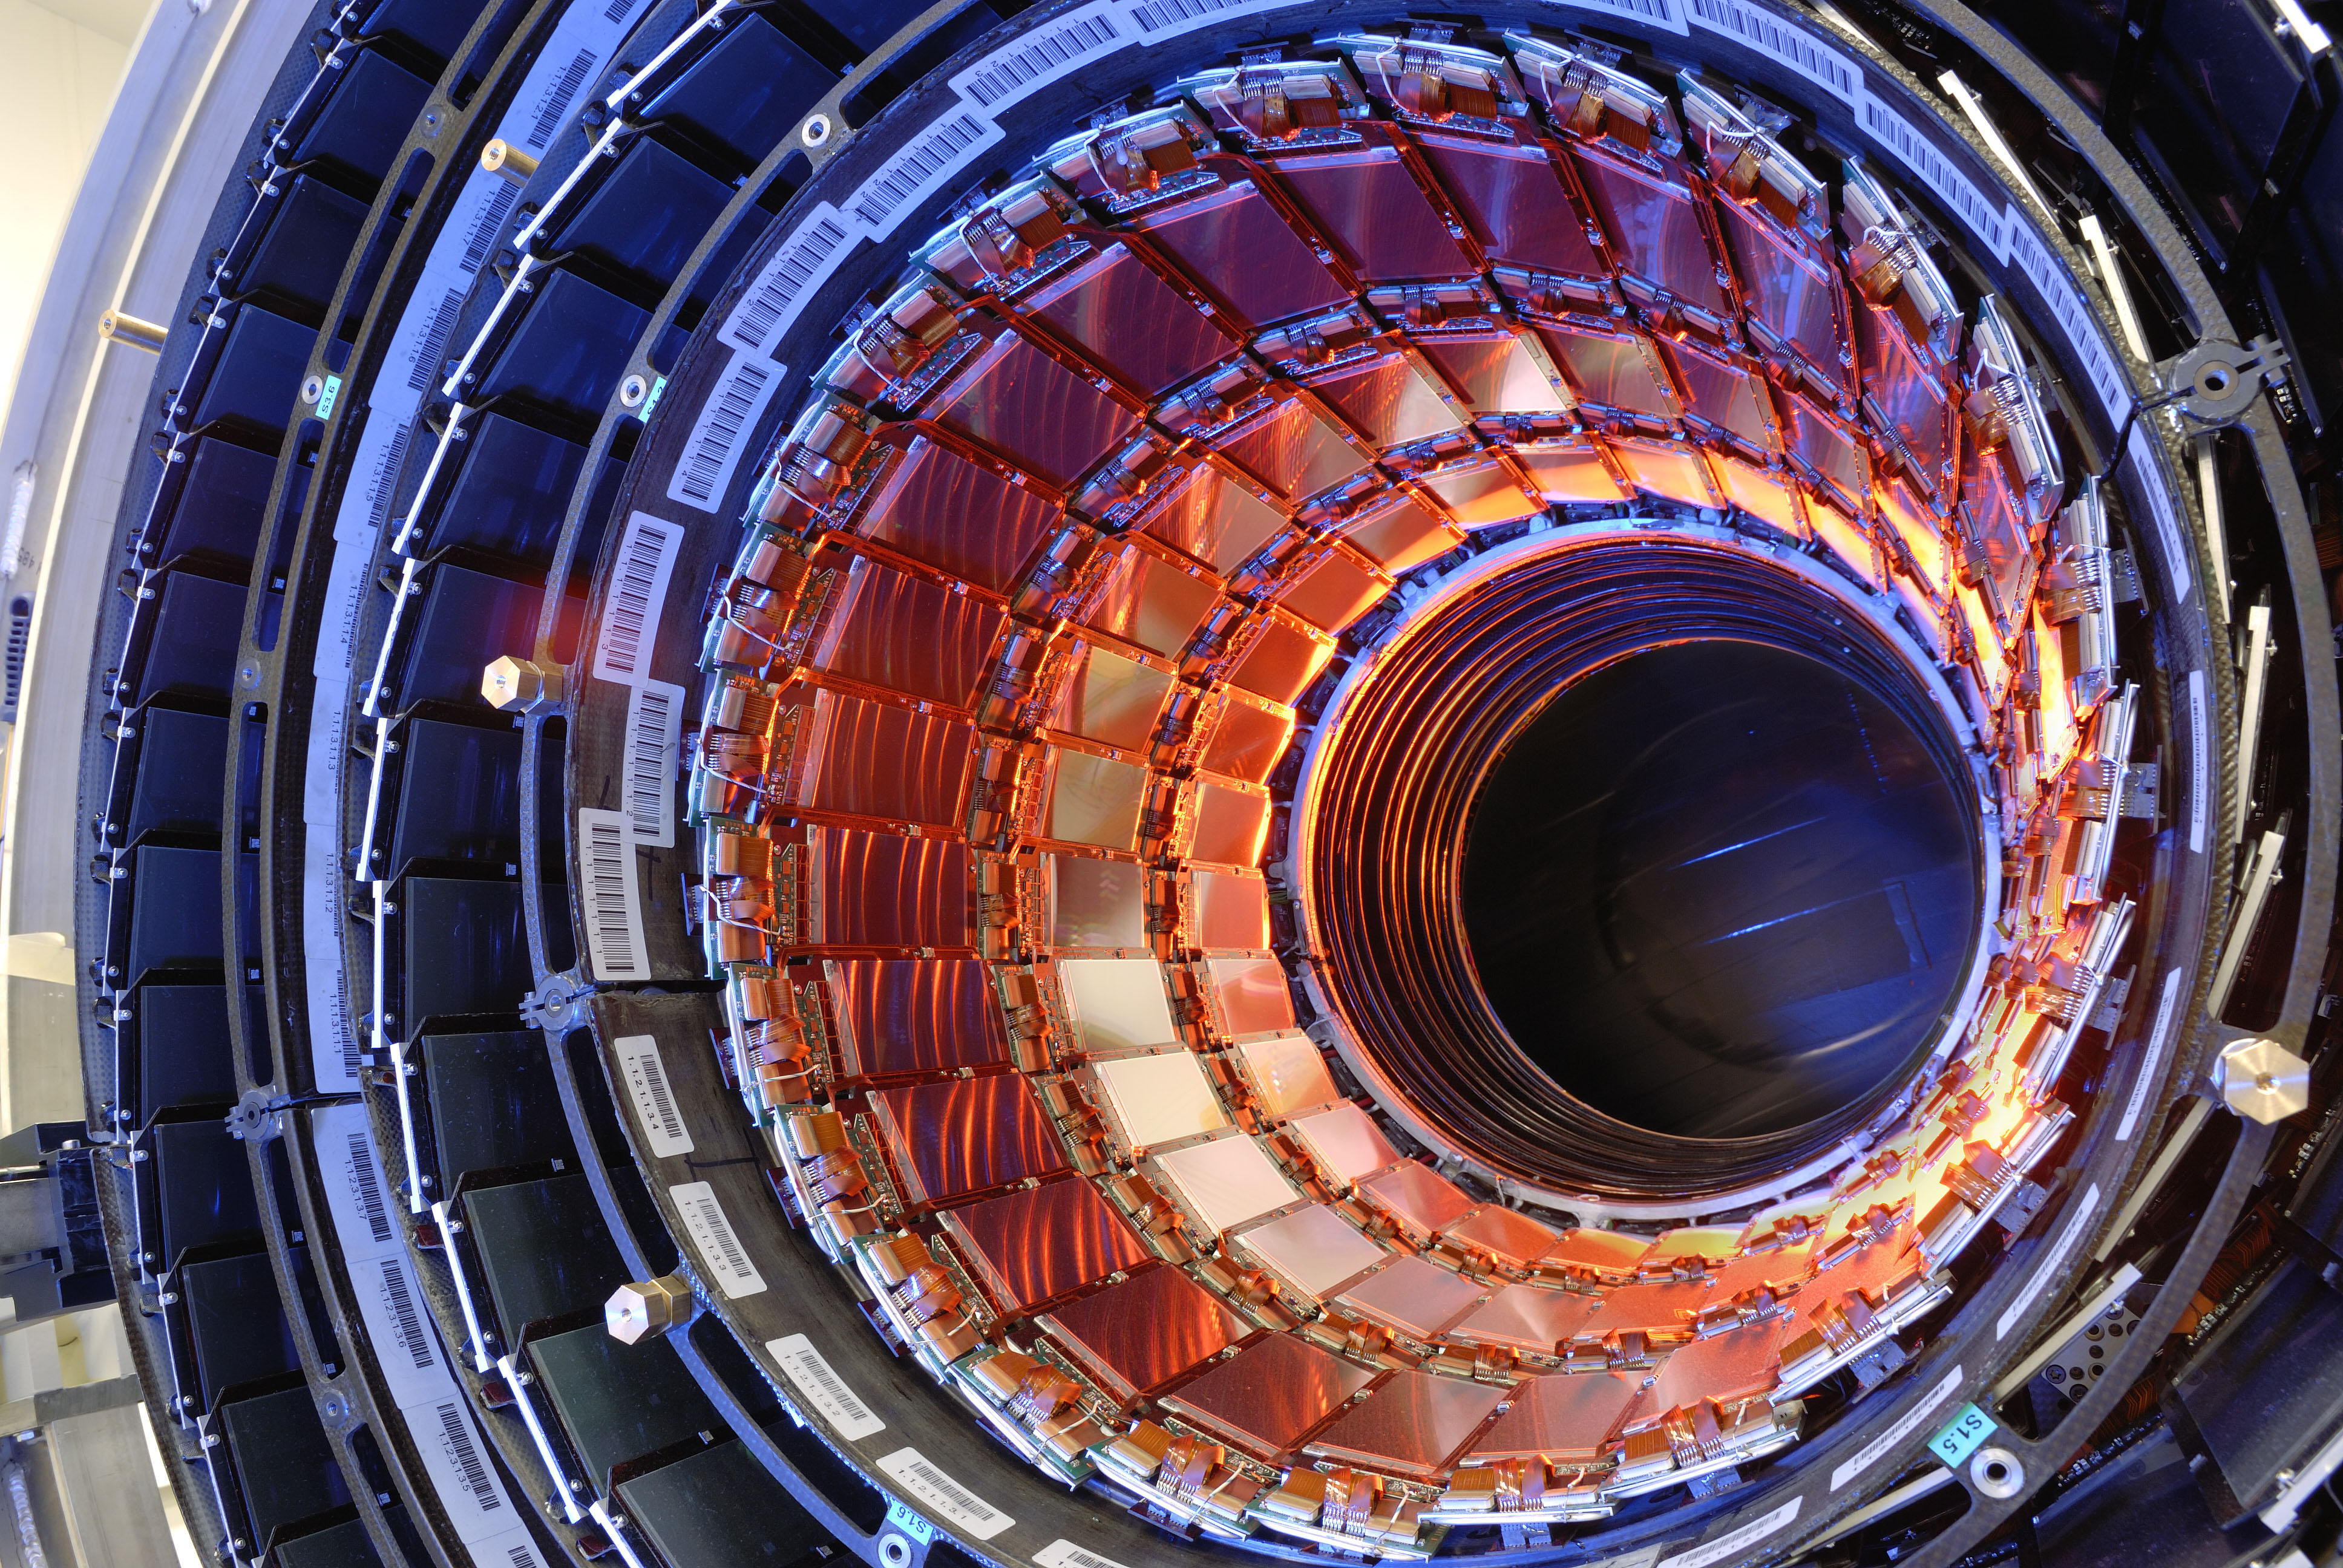
\includegraphics[width=0.70\linewidth]{Experiment/CMS/Image/Tracker/cms_track.jpg}}
  \hfil
  \subfigure[The position of silicon tracker on both sides of the IP ($z$ = 0\unit{cm}) \cite{Chatrchyan:2014fea}. 
	The pixel trackers are very close to the IP. For the strip tracker,
	there are tracker inner barrel (TIB), tracker outer barrel (TOB)
	in the barrel region, tracker endcap (TEC), and tracker inner disk (TID)
	in the transition region. The black (blue) lines correspond to single 
	(double) sided silicon strips. 
  \label{subfig:cms_track_pos}]
  {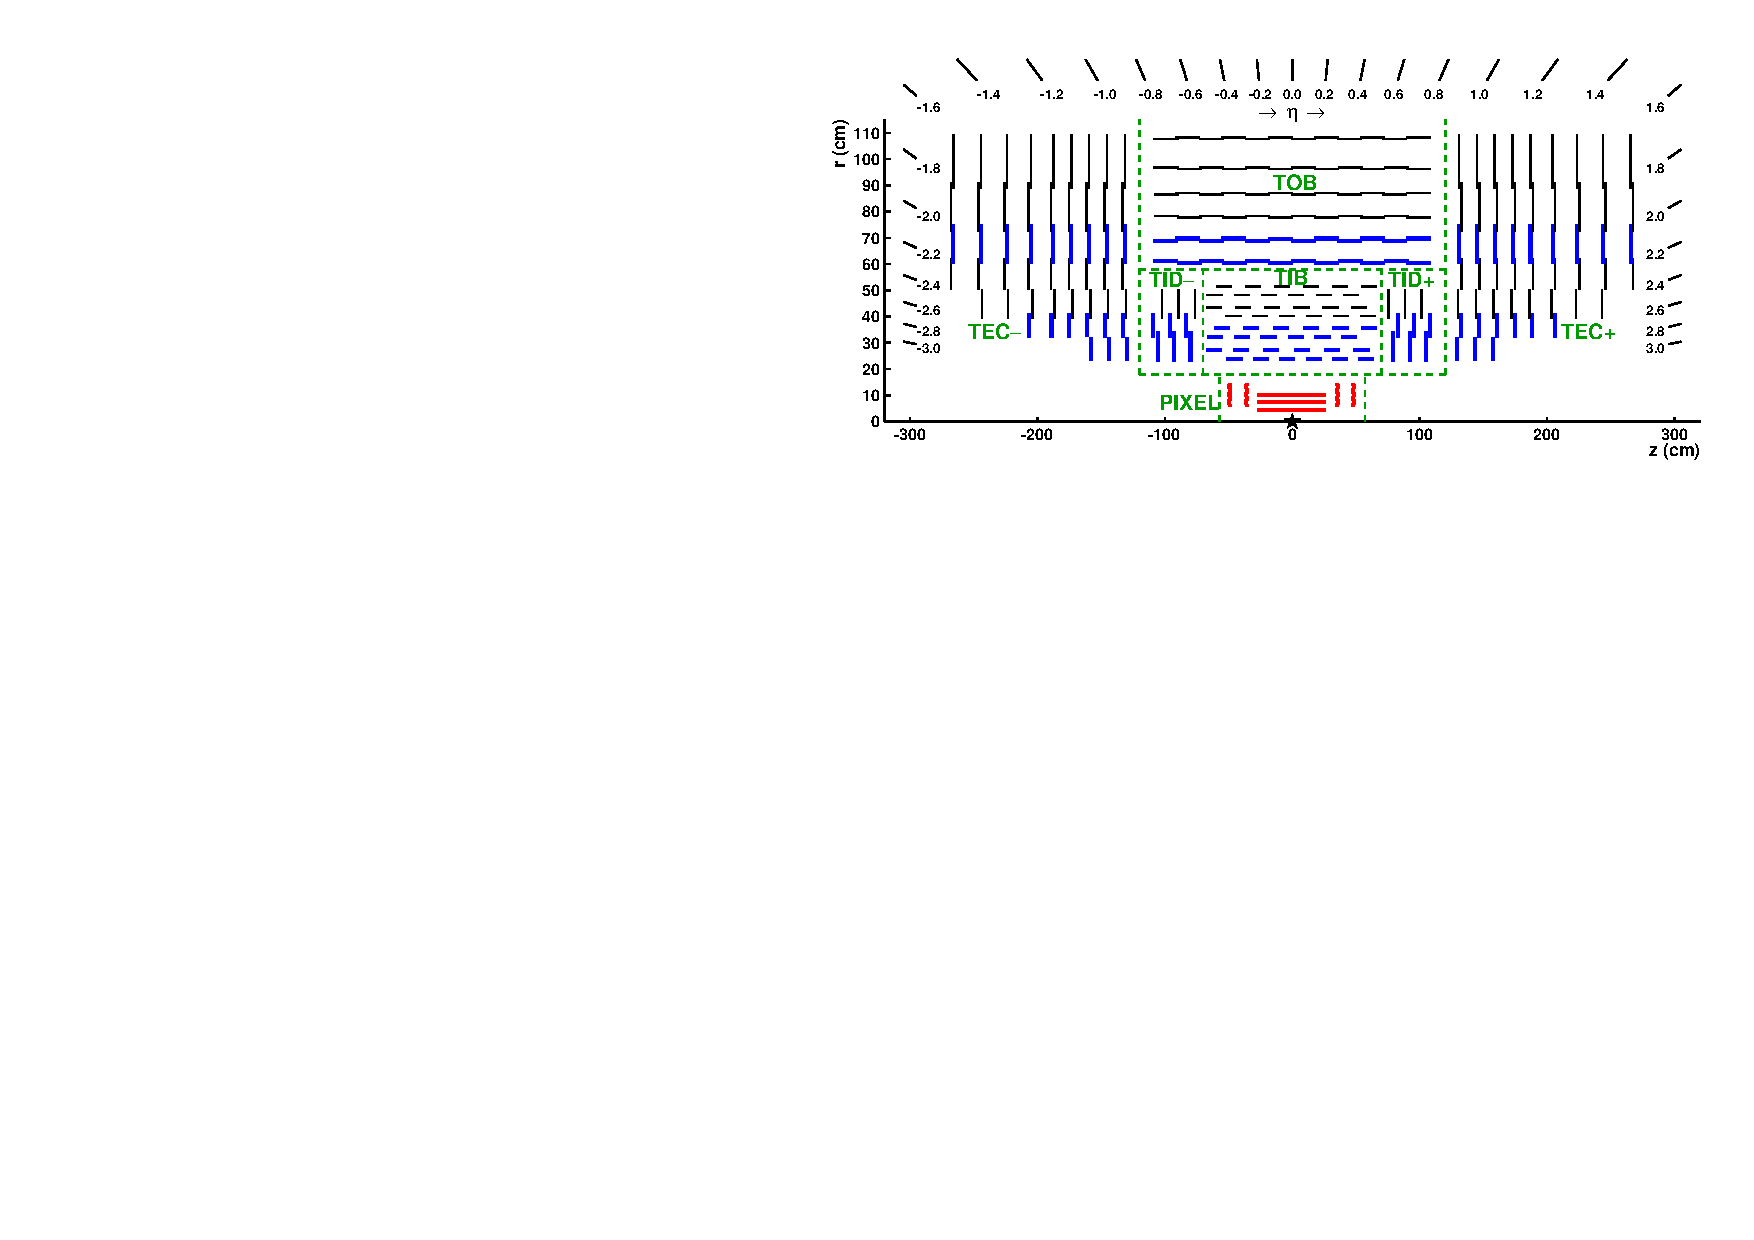
\includegraphics[width=0.90\linewidth]{Experiment/CMS/Image/Tracker/TrackerLayoutNew.pdf}}
  \caption{The silicon tracker of the CMS. The picture of one of trackers 
	inner barrel is shown in (a). The radial and $\eta$ position of the various
	parts of the pixel and strip tracker is shown in (b).}
  \label{fig:cms_tracker}
\end{figure}

The silicon detector is a reverse biased \rm{pn} junction, whose principle of operation 
is shown in Figure~\ref{fig:cms_diode}. Under the reverse 
bias voltage (80V), when a particle (for example, a minimum ionising particle) traverses 
through the bulk n-type region, several electron-hole pairs ( about 24,000) are created in 
the depletion region. The electrons, thus created, are attracted towards the $\rm p^+$ 
implant due to the applied electric field within very short time of about 10 ns.
The electrons collected at $\rm p^+$ implant are amplified and readout by the backend electronics.
\begin{figure}
  \begin{center}
	  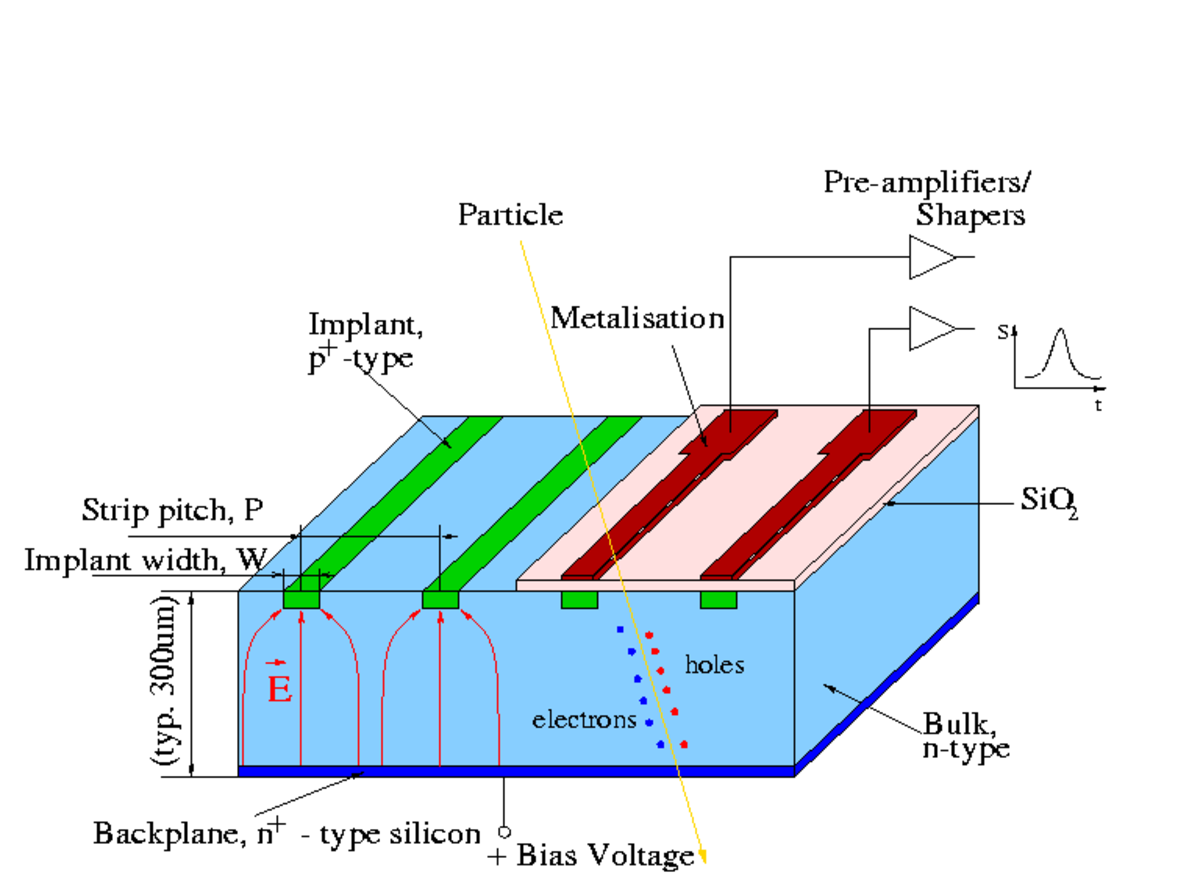
\includegraphics[width=0.75\linewidth]{Experiment/CMS/Image/Tracker/cms_diode.pdf}
  \caption{The principle of operation of a silicon detector \cite{Diode}. The green
	  strips are $\rm p^+$ -type of semiconductor where the electrons are 
	  attracted after being produced in the depletion region when a particle
	  passes through. The $\rm{SiO}_2$ layer along with metallic surface, on top of 
	  the green strips, provides conducting circuits for the electron. The 
	  amplifiers/shapers are used to amplify and shape the electron current.
	  The holes are attracted towards the $+ve$ bias voltage.}
  \label{fig:cms_diode}
  \end{center}
\end{figure}

As alluded earlier, the CMS silicon tracker is divided into two types:
\begin{itemize}[leftmargin=*]		
\item $\textbf{Pixel tracker}$:
	The innermost component of the tracker, the pixel detector occupies the central 
	region close to which the collision happens. It operates in a 
	high-radiation environment. The length of the pixel detector from 
	interaction point along the beam axis is 46.5\unit{cm}, while two endcaps are placed 
	at $z$ = 34.5 and 46.5\unit{cm} from both sides of the IP. The 3-layers of the detector
	are placed at r = 4.4, 7.3, and 10.2\unit{cm} in the barrel region as shown in 
	Figure~\ref{fig:cms_pixel}. 
	\begin{figure}
	  \centering
		\subfigure[Pixel layers \cite{Chatrchyan:2009aa} 
	  \label{subfig:cms_pixel}]
	  {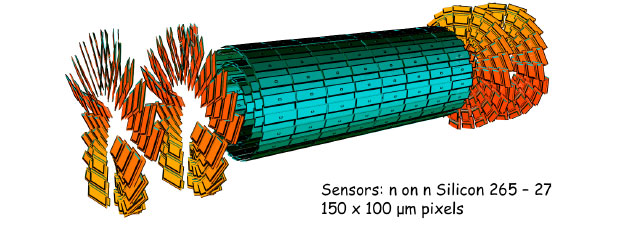
\includegraphics[width=0.50\linewidth]{Experiment/CMS/Image/Tracker/pixel.png}}
	  \hfil
	  \subfigure[Locations of pixel layers \cite{Veszpremi:2014exa}. 
	  \label{subfig:pixel_pos}]
	  {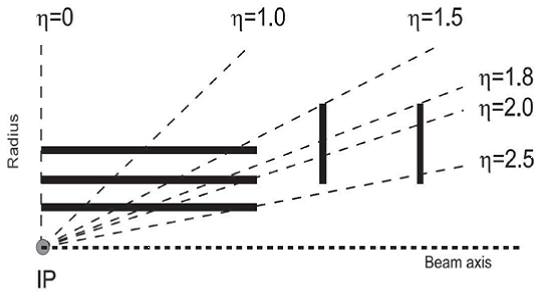
\includegraphics[width=0.40\linewidth]{Experiment/CMS/Image/Tracker/pixel2.png}}
	  \caption{The pixel detector of the CMS tracker. The location of pixel layers 
		in the barrel and endcap region is shown in (b).}
	  \label{fig:cms_pixel}
	\end{figure}
\item $\textbf{Strip tracker}$:
	The major part of the tracker is covered by the silicon strip detectors 
	as shown in Figure~\ref{fig:cms_tracker}. The length of strip detectors
	is 5.8\unit{m}, and diameter is 2.5\unit{m}. There are over 15000 modules covering 
	$0 \geq \eta \geq 2.5$. The charge generated, when a particle passes 
	through the strip detectors, is read and amplified from each micro-strip 
	as shown in Figure~\ref{fig:cms_diode}. 
\end{itemize}

The total thickness of tracker material in units of radiation length (it is a characteristic 
of a material defined as the distance traveled by an electron when it
loses $1/e$ of its energy due to the Bremsstrahlung radiation) and nuclear interaction length
(it is the mean distance a hadronic particle travels before undergoing an inelastic
nuclear interaction) is shown in Figure~\ref{fig:cms_track_budget}. In the direction
perpendicular to the $z$-axis ($\eta = 0$), the thickness is small ($t/X_0 \approx 0.4$).
That is, an electron produced at collision point can traverse in the $\eta = 0$ 
direction by losing only 14.7\% (0.4/2.718) of its initial energy. The thickness is 
maximum in the endcap region as shown in Figure~\ref{fig:cms_track_budget}.
\begin{figure}
  \centering
  \subfigure[Thickness in units of radiation length]
  {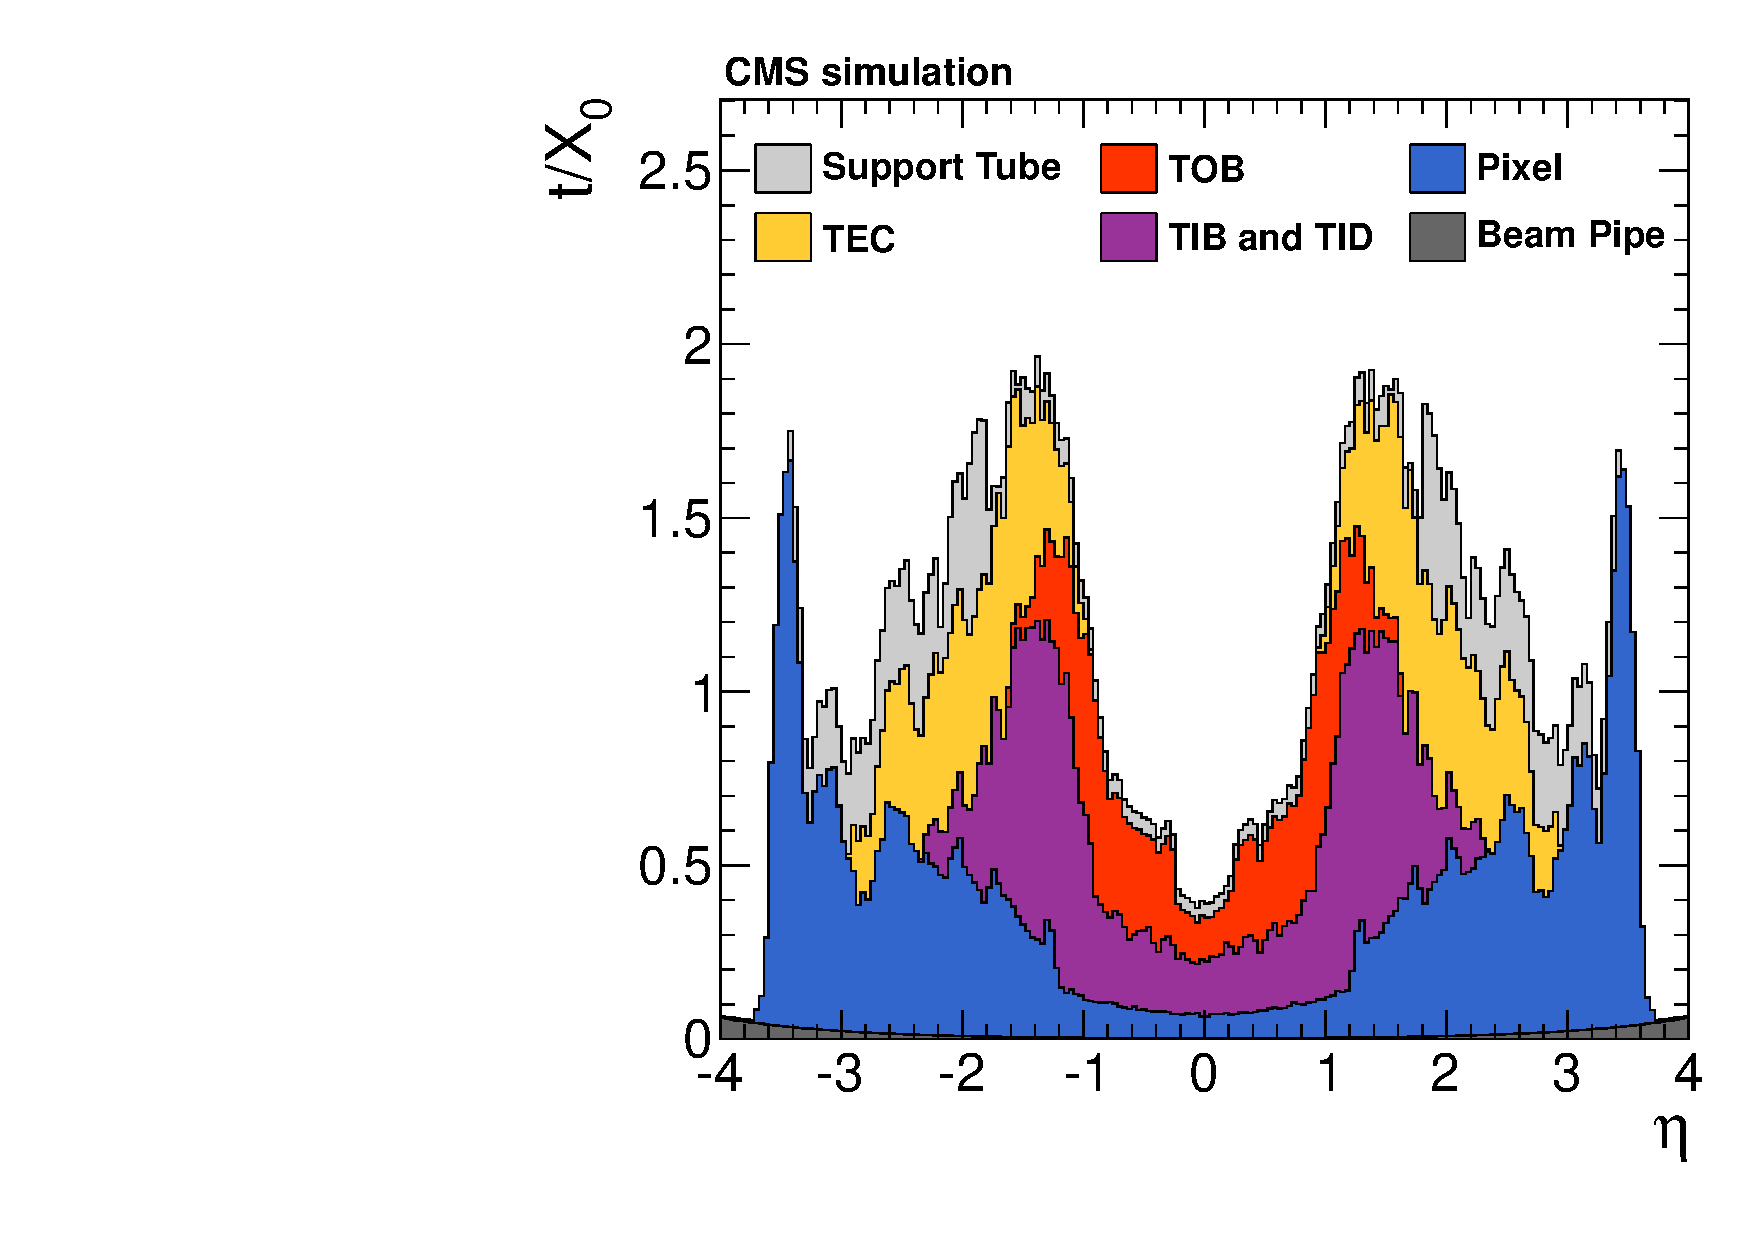
\includegraphics[width=0.49\linewidth]{Experiment/CMS/Image/Tracker/MaterialBudget_RadLengths.pdf}}
  \hfil
  \subfigure[Thickness in units of interaction length]
  {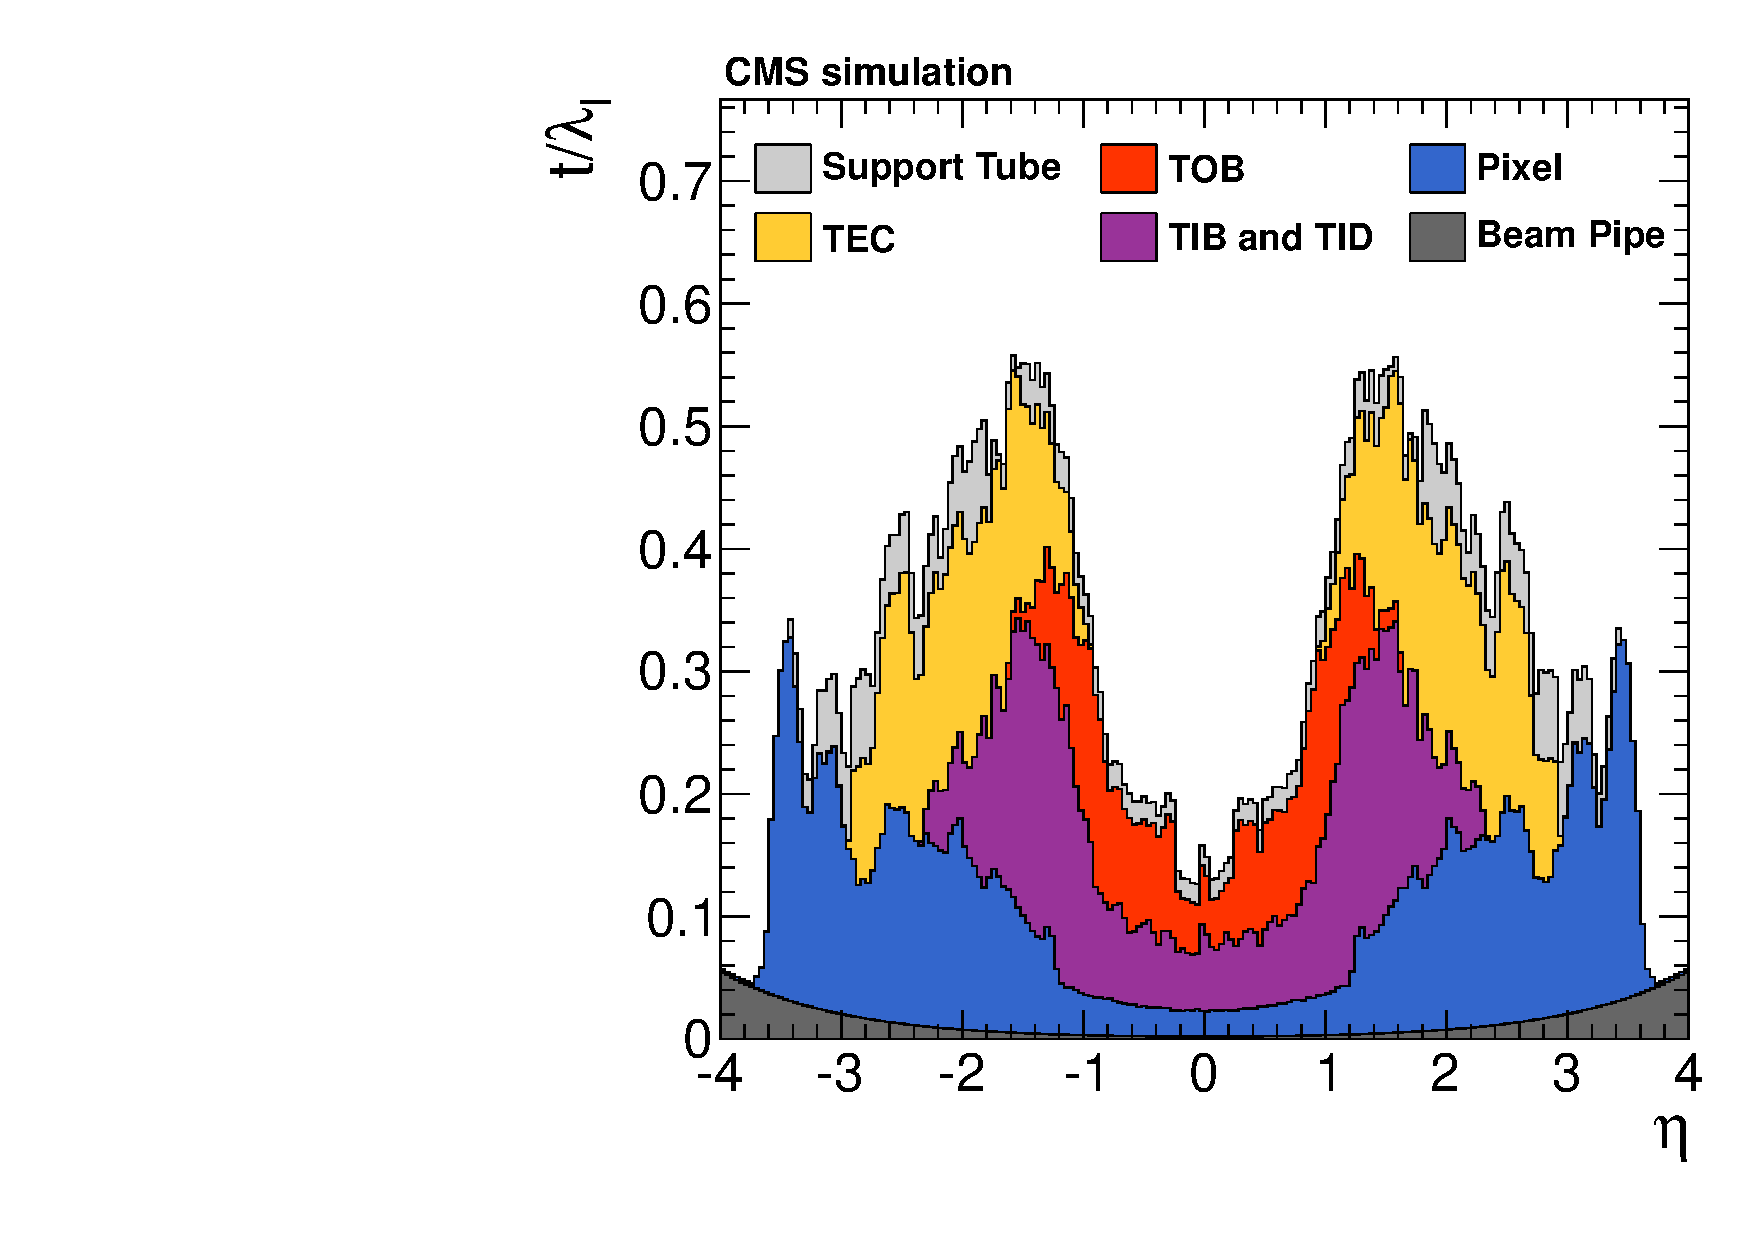
\includegraphics[width=0.49\linewidth]{Experiment/CMS/Image/Tracker/MaterialBudget_InteractionLengths.pdf}}
  \caption{Total thickness of the silicon tracker in units of radiation and interaction 
	lengths \cite{Chatrchyan:2014fea}. The thickness of supporting tube and beam 
	pipe is also shown.}
  \label{fig:cms_track_budget}
\end{figure}

The resolution is the parameter that characterizes how accurately a measurement
is performed. For example, if a detector \dq{measures} the momentum of a particle
to be 100 \GeV and the momentum \dq{resolution} is 5 \GeV then it implies that the 
\dq{actual} value of the momentum would be in the range of 95 to 105 \GeV. Hence lower the 
value of detector resolution, the more precise is the measurement. The absolute 
(relative) resolution of $\phi$ (\pt) of the silicon tracker as a function of $\eta$
is shown in Figure~\ref{fig:cms_track_reso_part} of muons, electrons, and charged
pions \cite{Chatrchyan:2014fea}. The $\eta$ and \pt resolution of all particles are 
better in the barrel region as compared to that in endcap regions. The resolution 
for muons is better as compared to electrons and charged pions in all regions. Also, 
the higher the \pt, better is the resolution for all charged particles. For \pt = 100 \GeV, 
the momentum resolution at $\eta$ = 0 is 2\%, 30\%, and 3\% for muons, electrons, and pions 
respectively.
The silicon tracker is essential for the reconstruction of trajectories of charged particles. 
Being very close to the collision point, these are also useful for high level triggering as discussed 
in Section~\ref{ss:secTrig}. 

\begin{figure}
  \centering
  \subfigure[]
  {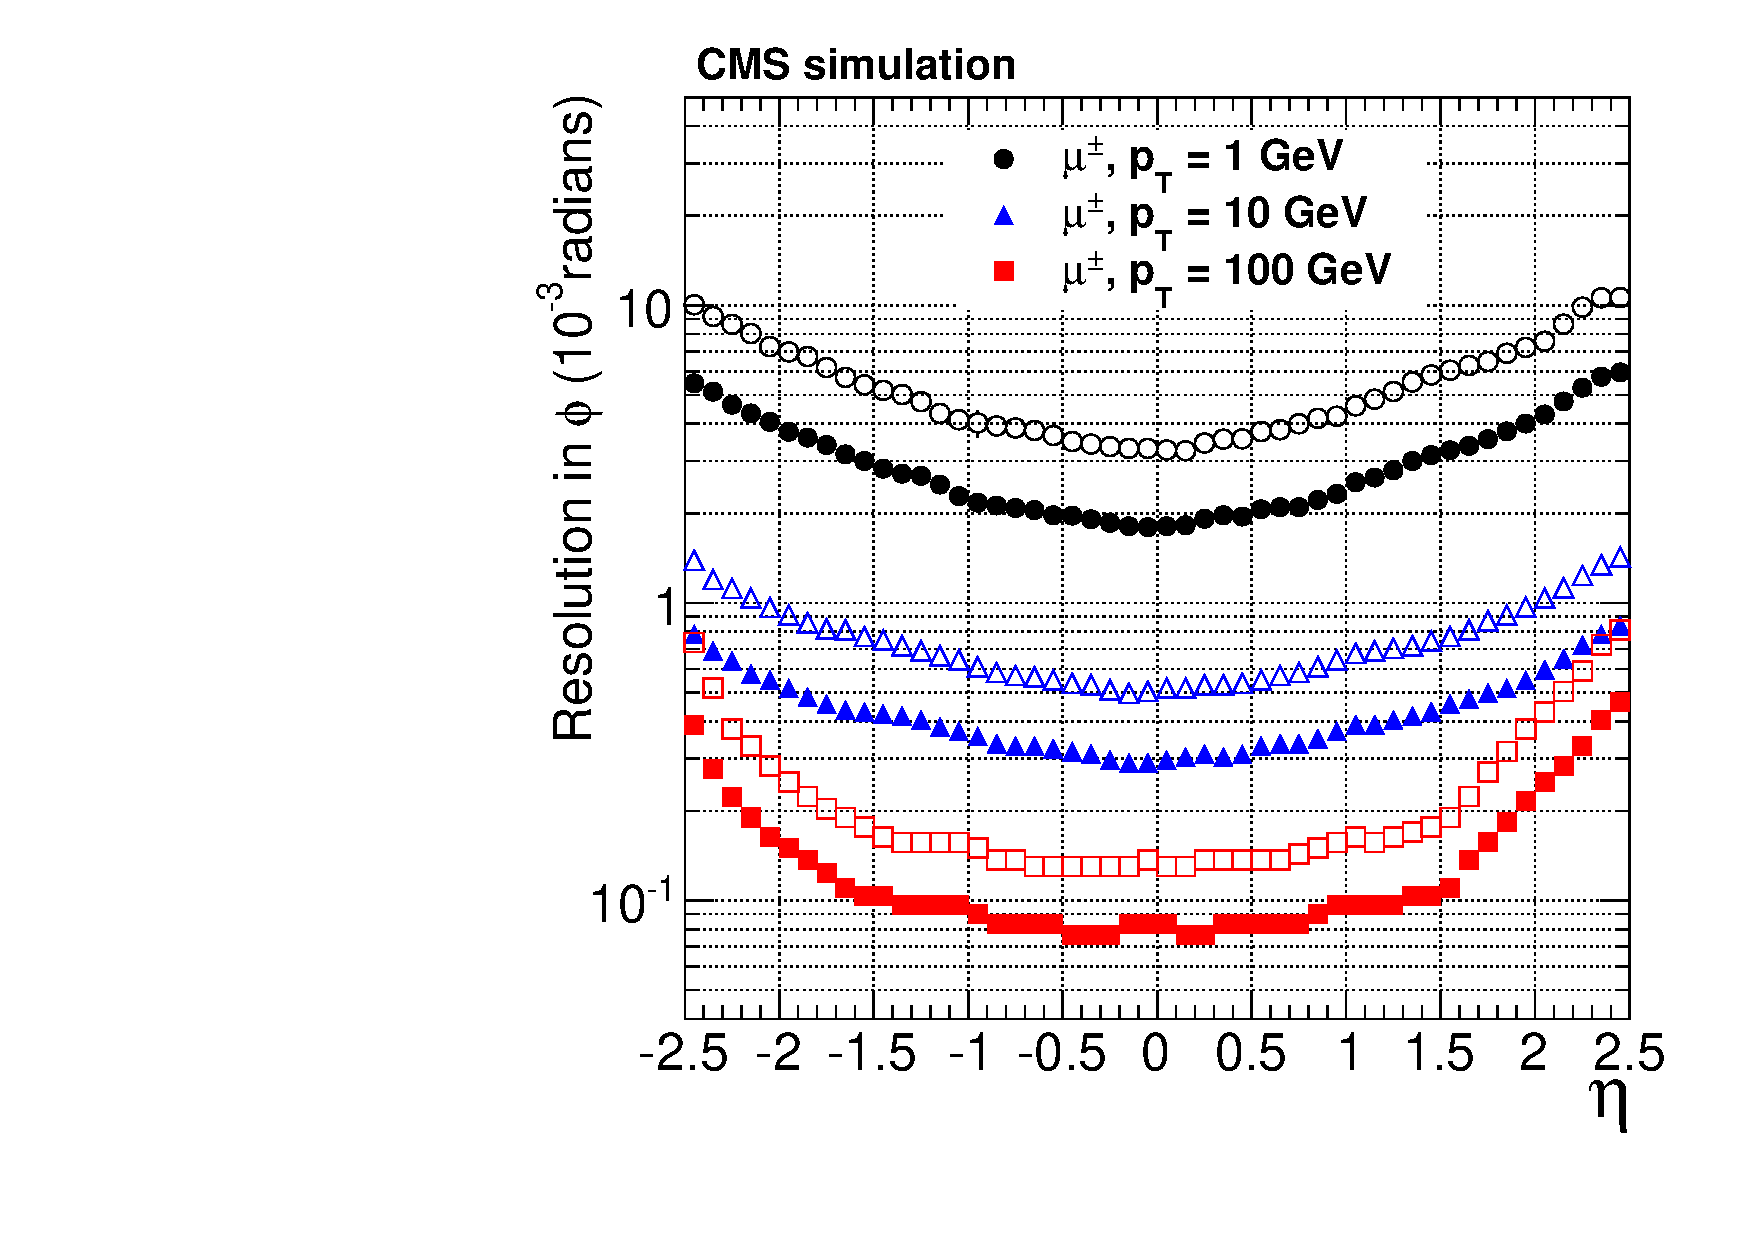
\includegraphics[width=0.40\linewidth]{Experiment/CMS/Image/Tracker/mu_resolutionPhiVsEta.pdf}}
  \subfigure[]
  {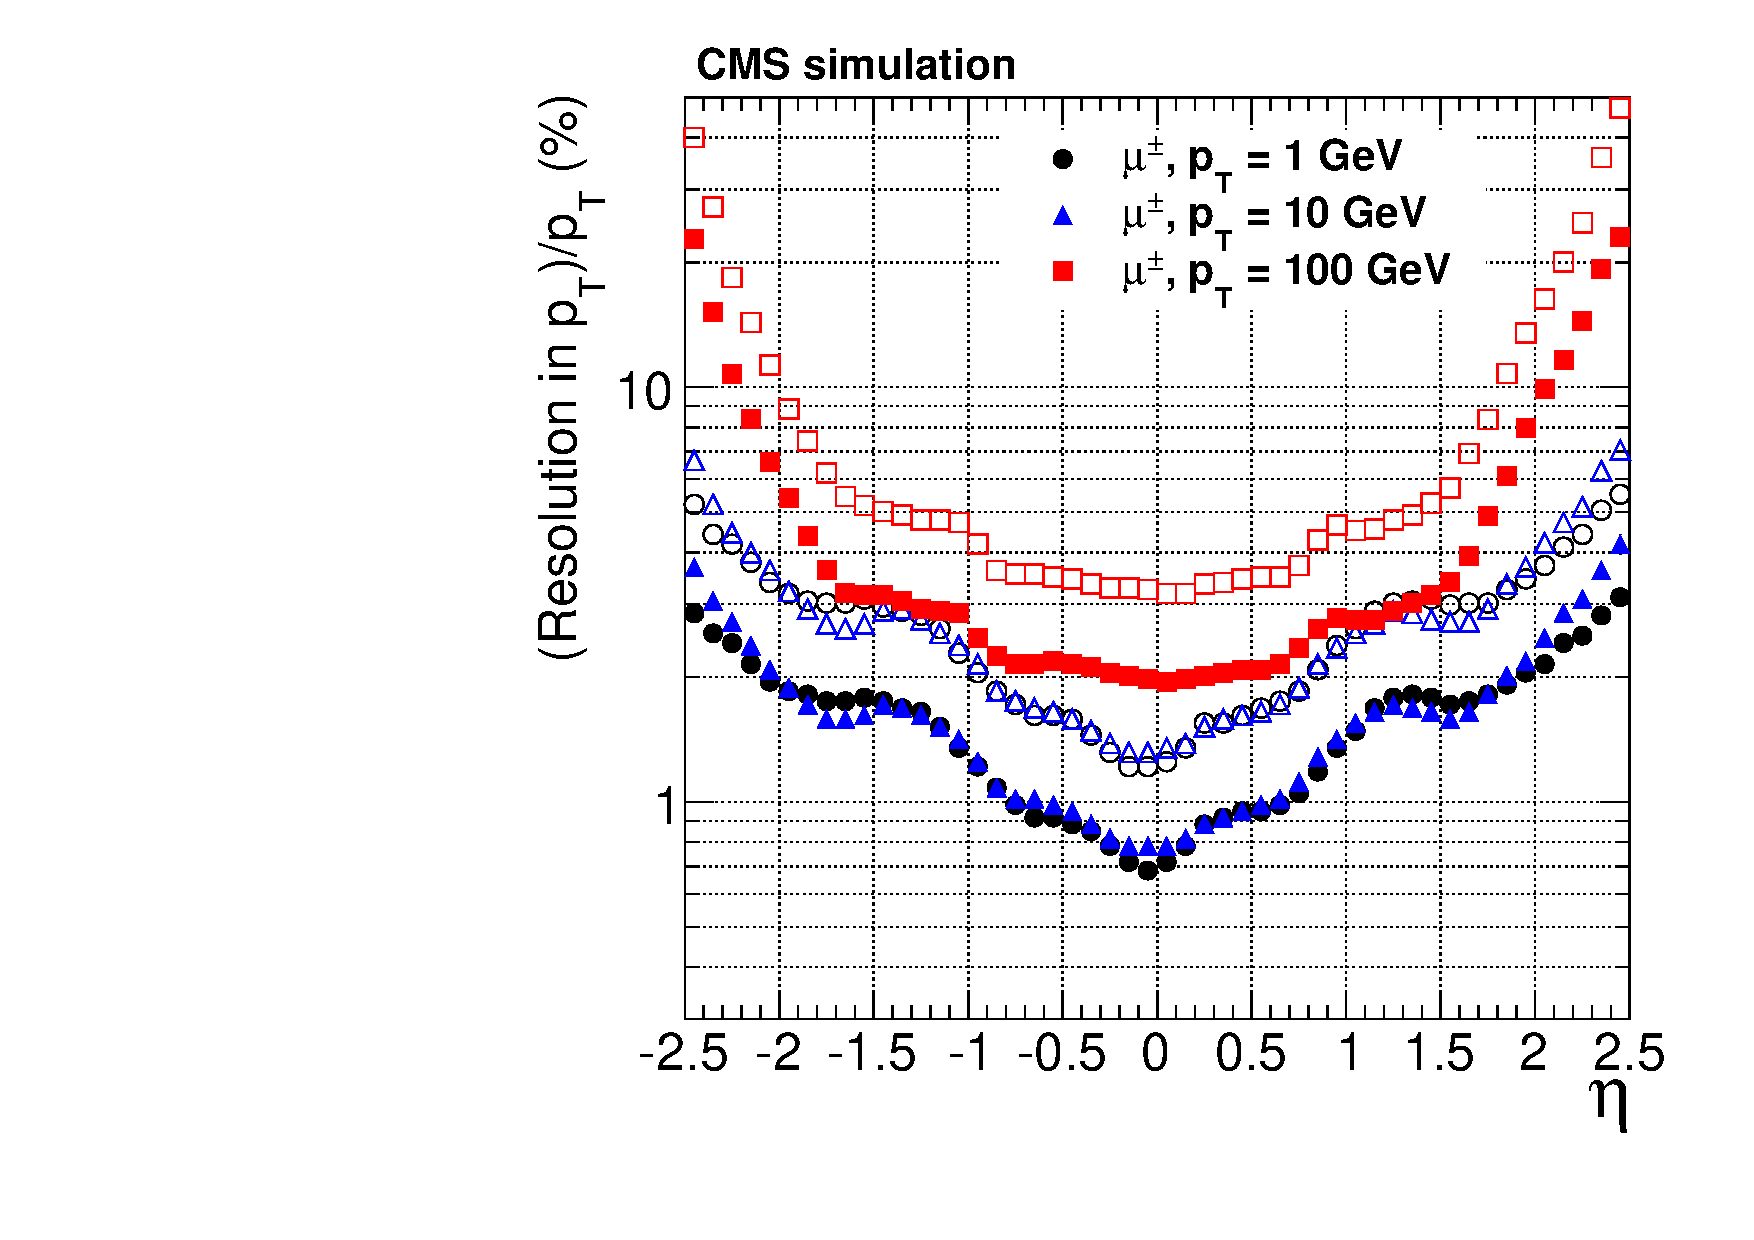
\includegraphics[width=0.40\linewidth]{Experiment/CMS/Image/Tracker/mu_resolutionPtVsEta.pdf}}
  \vfil
  \subfigure[]
  {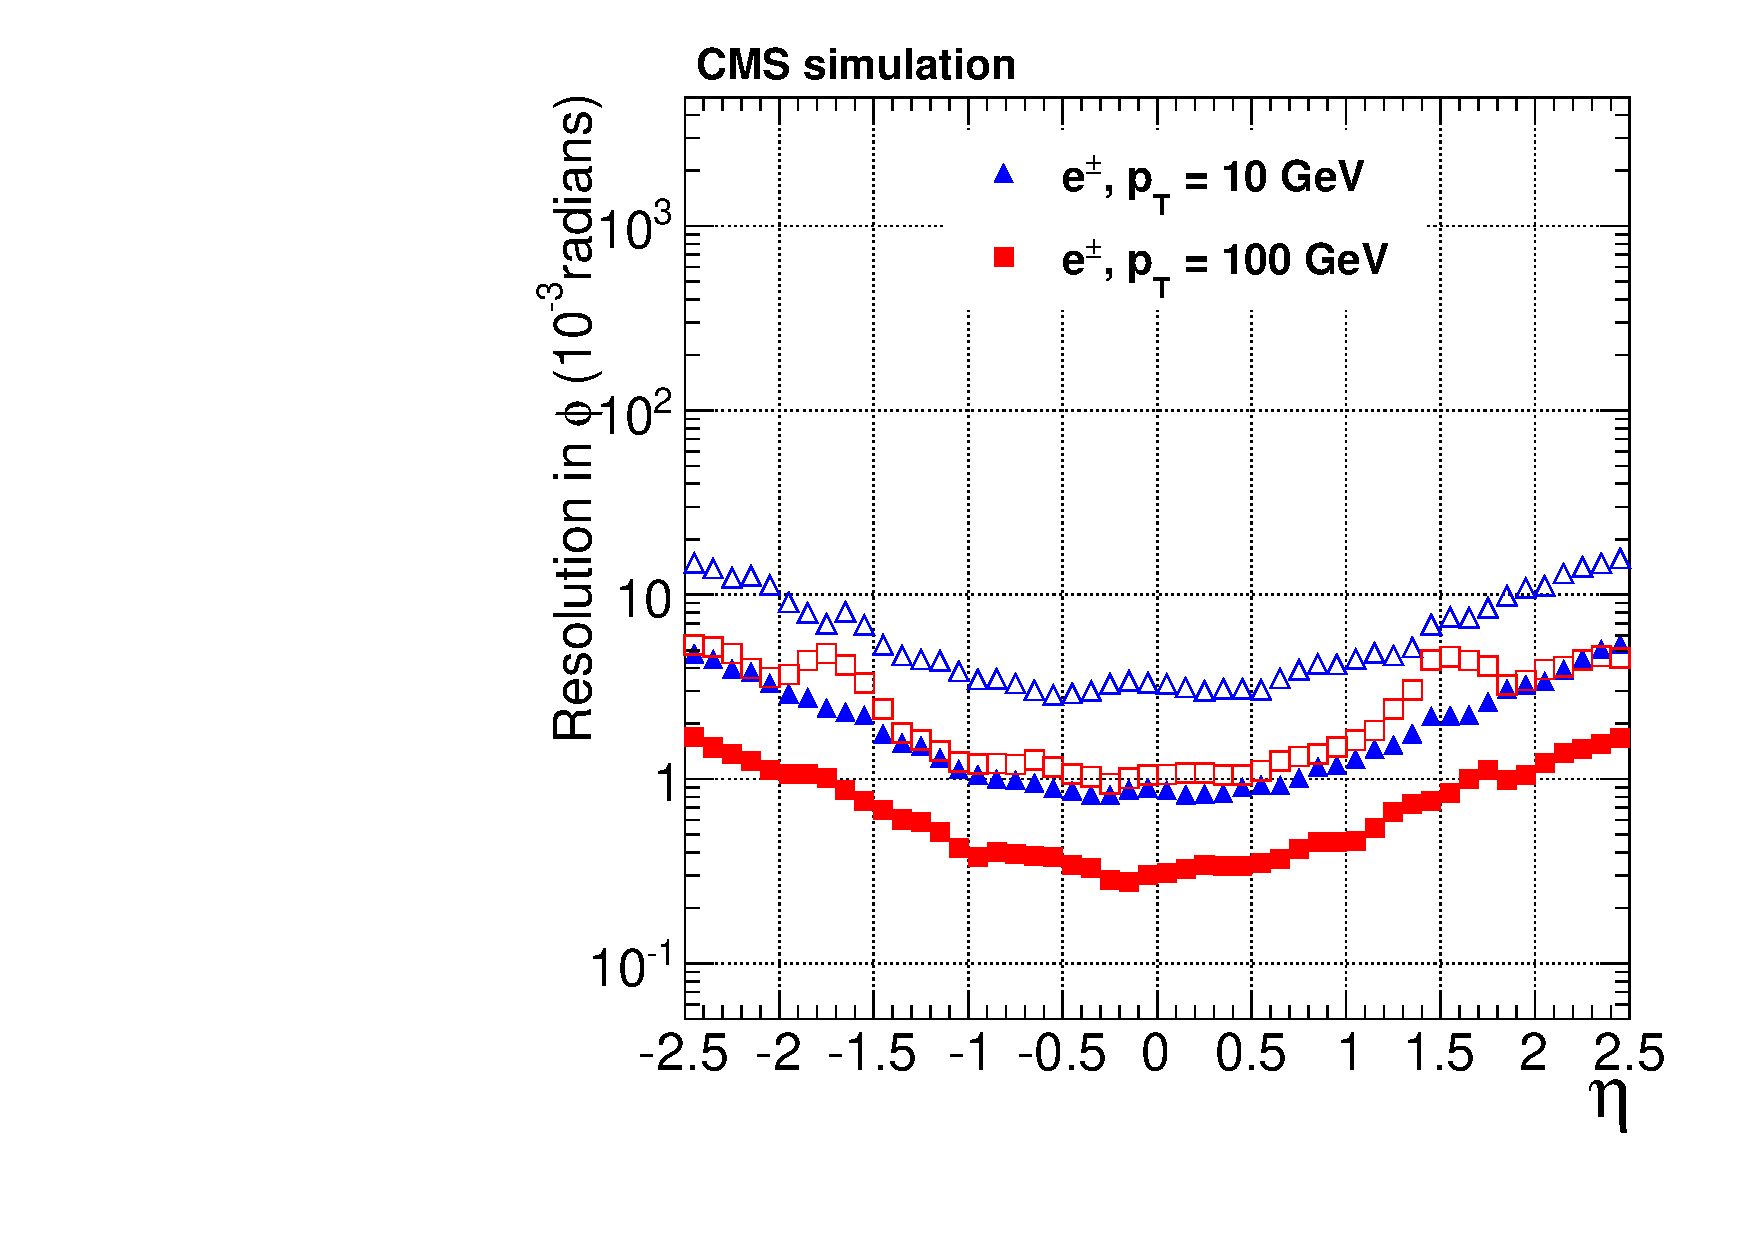
\includegraphics[width=0.40\linewidth]{Experiment/CMS/Image/Tracker/ele_resolutionPhiVsEta.pdf}}
  \subfigure[]
  {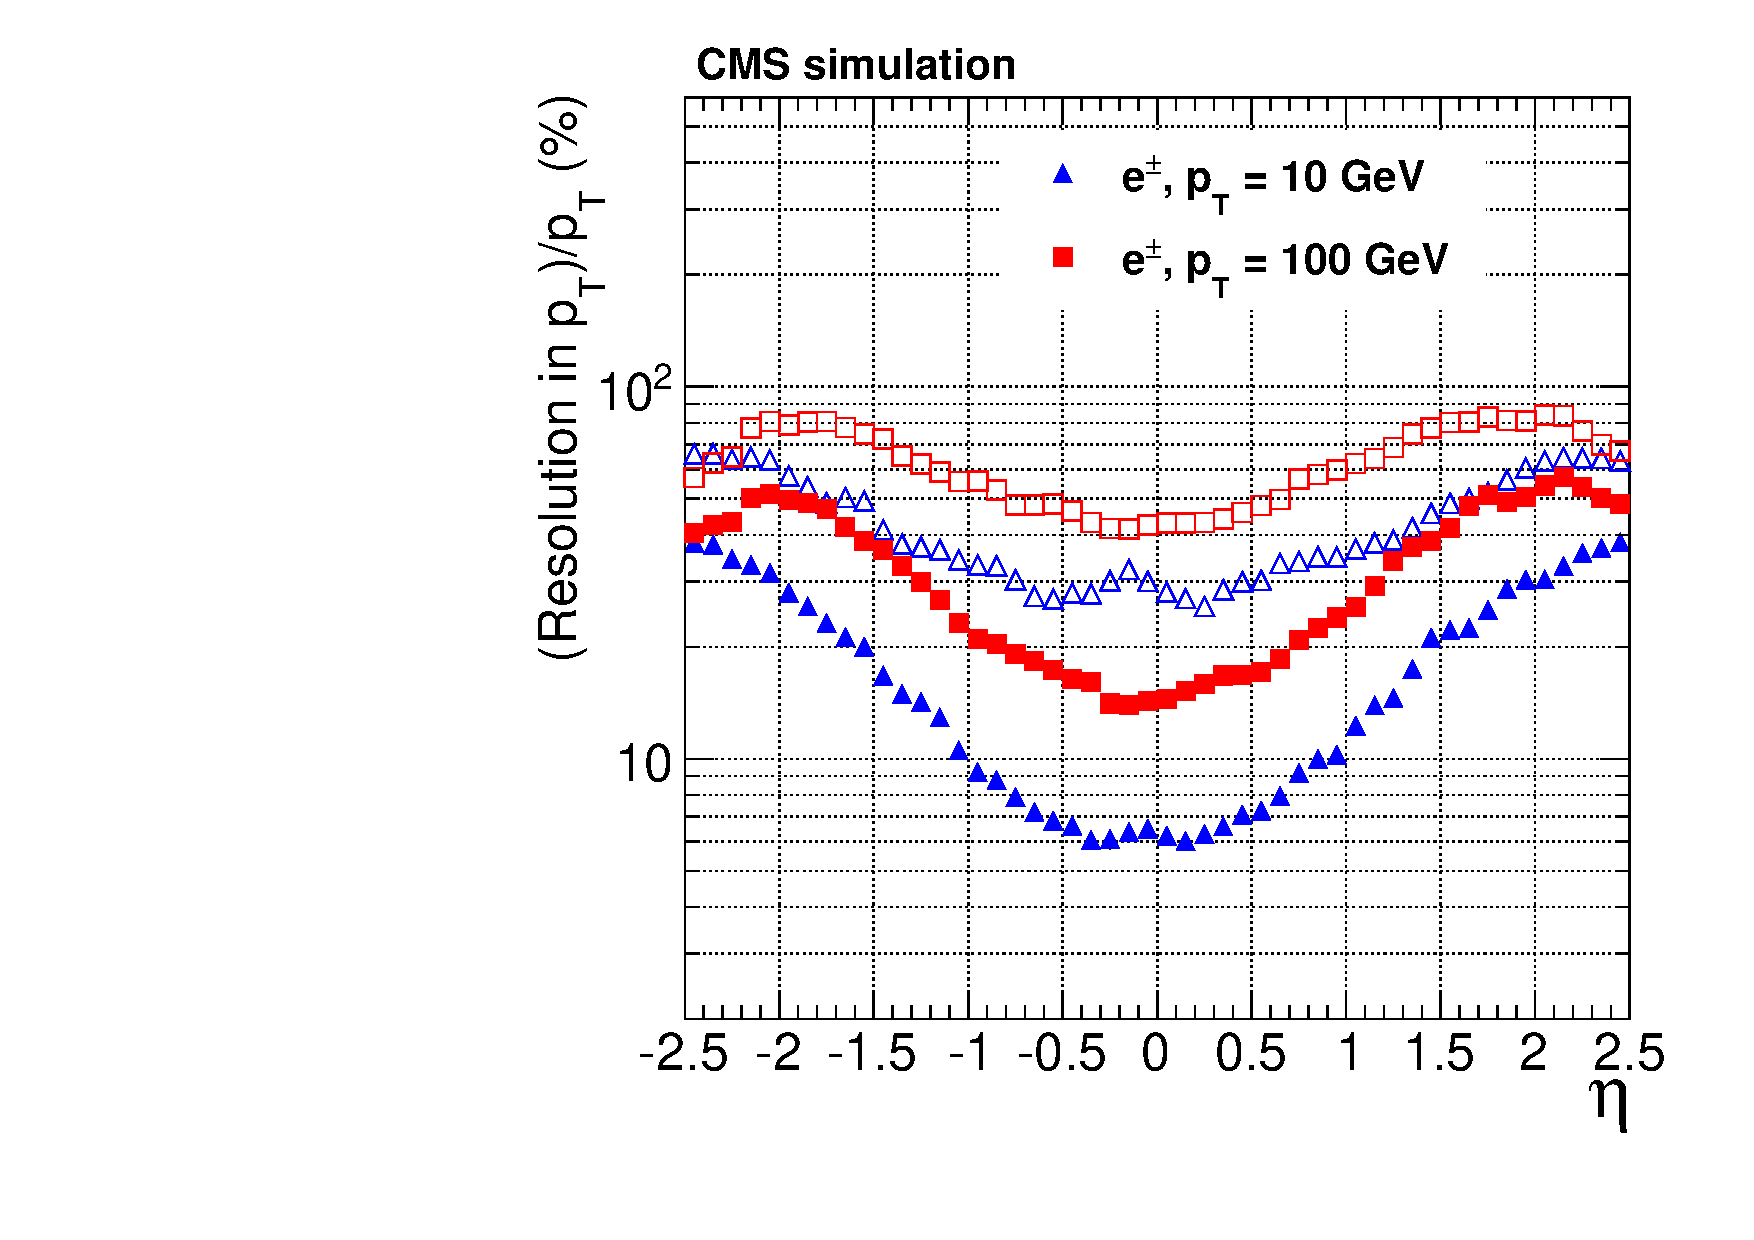
\includegraphics[width=0.40\linewidth]{Experiment/CMS/Image/Tracker/ele_resolutionPtVsEta.pdf}}
  \vfil
  \subfigure[]
  {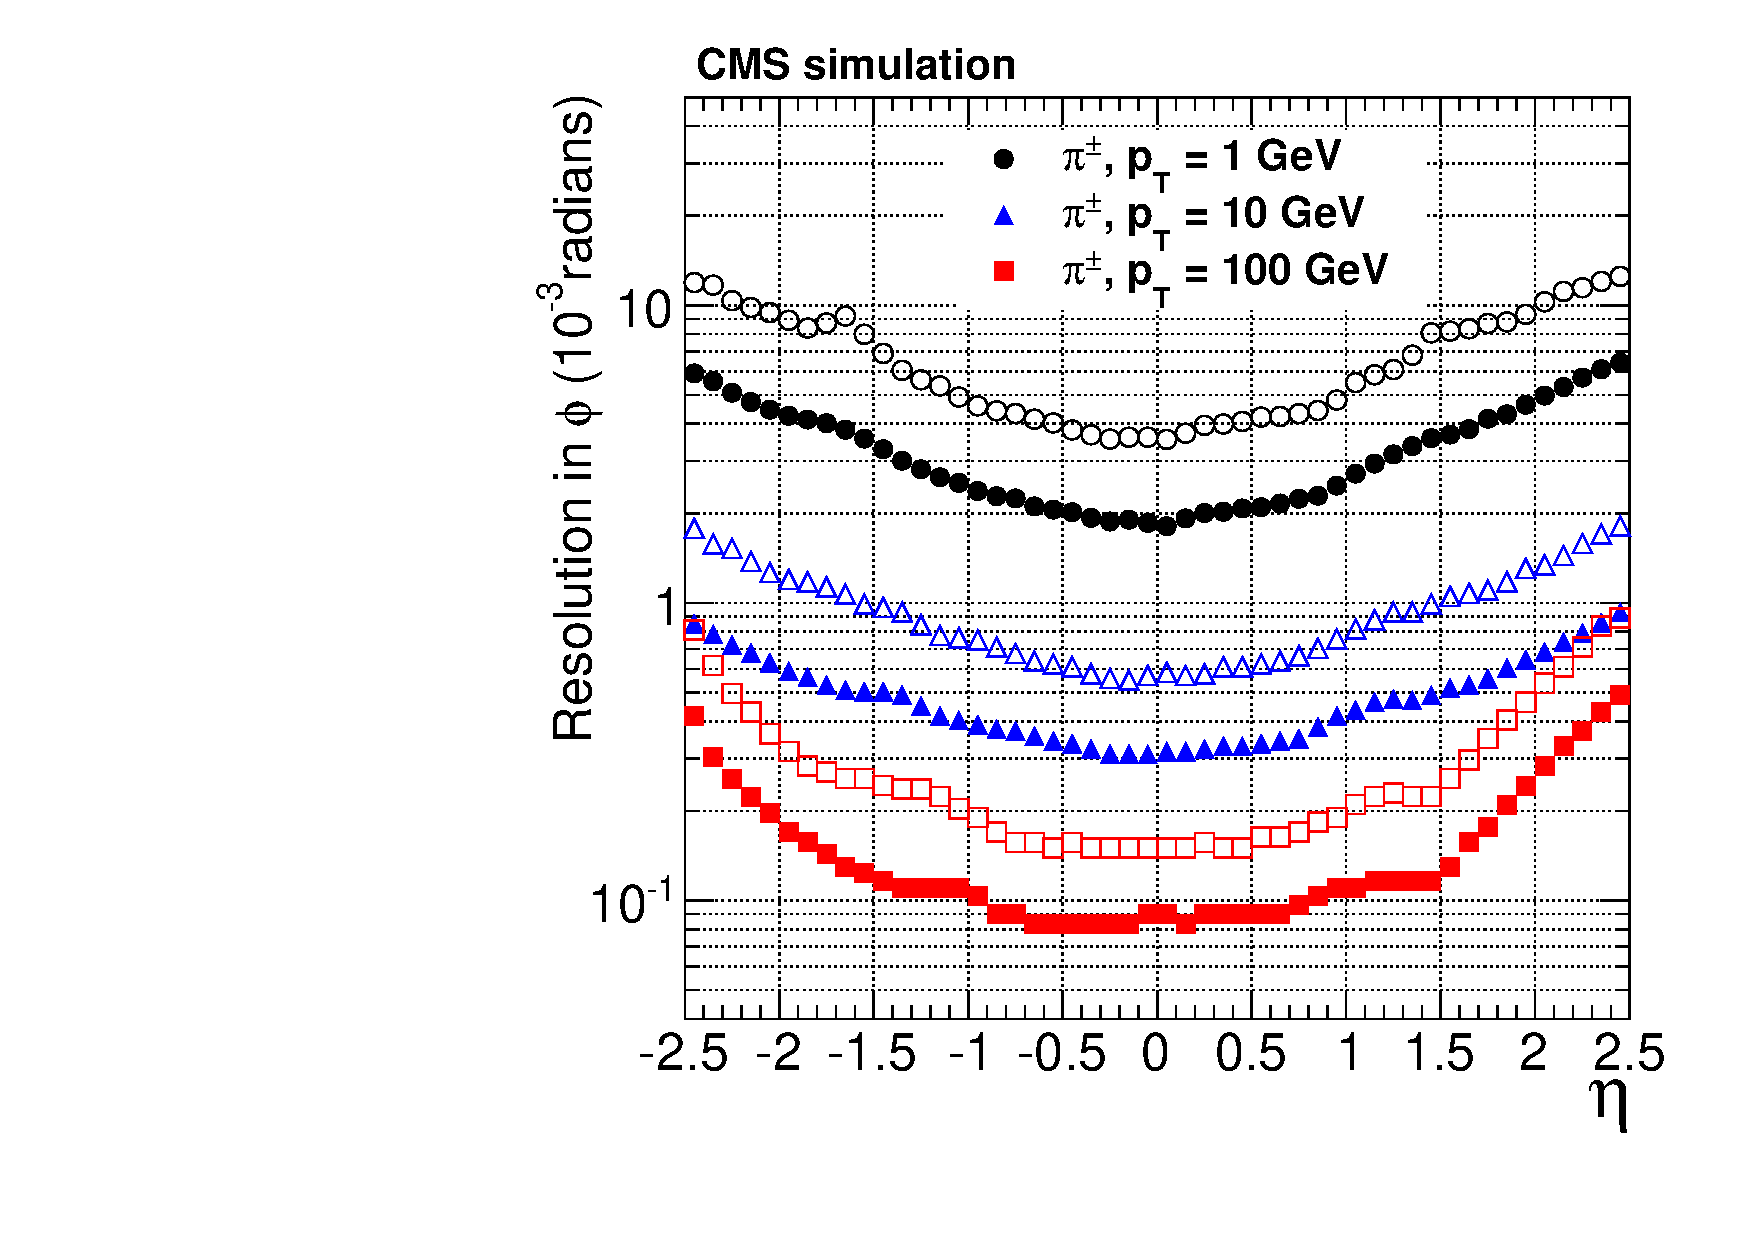
\includegraphics[width=0.40\linewidth]{Experiment/CMS/Image/Tracker/pi_resolutionPhiVsEta.pdf}}
  \subfigure[]
  {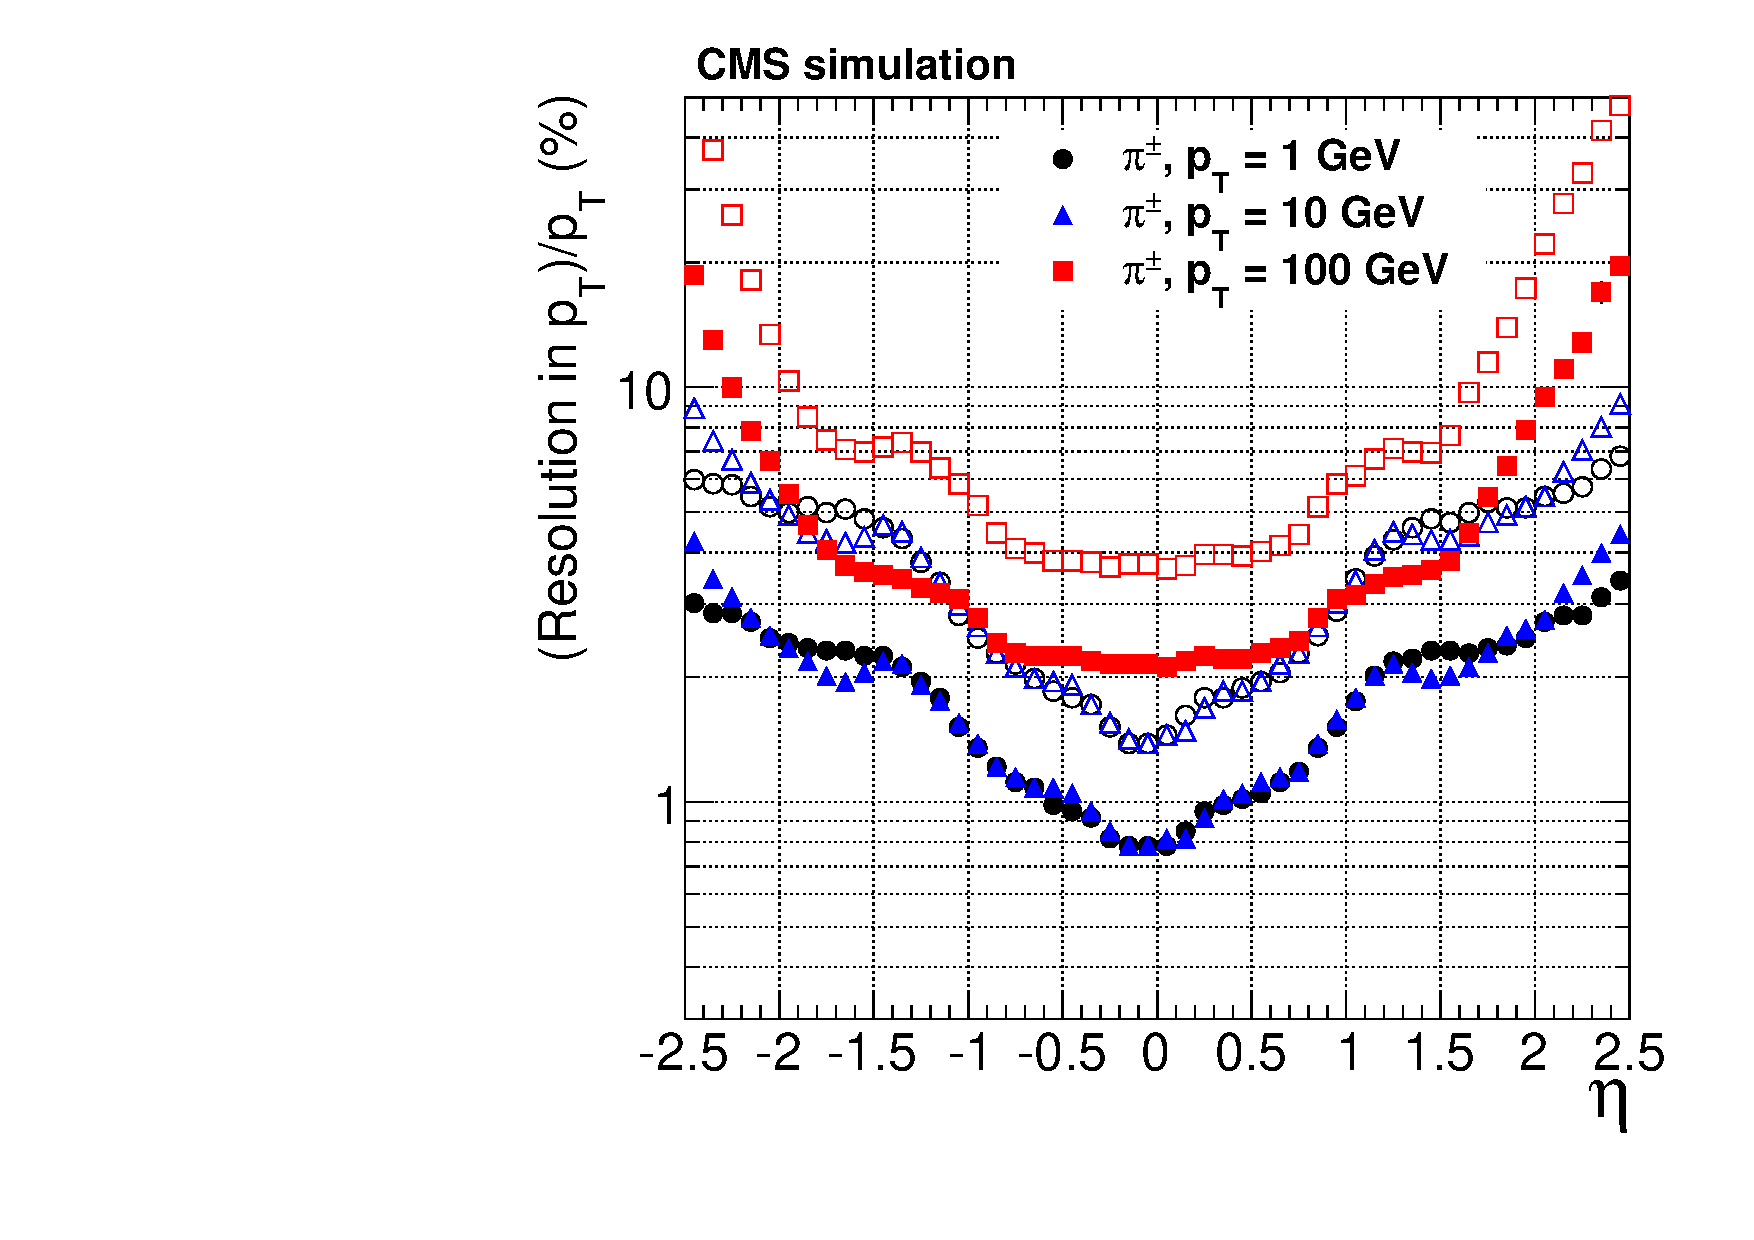
\includegraphics[width=0.40\linewidth]{Experiment/CMS/Image/Tracker/pi_resolutionPtVsEta.pdf}}
  \caption{The absolute resolution of $\phi$ and relative resolution of \pt measurement
  of muons, electrons, and charged pions from the silicon tracker as function of 
  $\eta$ \cite{Chatrchyan:2014fea}. Other resolution such as $d_0, z_0$, 
  and $\cot\theta$ are given in Reference~\cite{Chatrchyan:2014fea}. The open (solid) markers 
  correspond to the half-width for 90\% (68\%) intervals \cite{Chatrchyan:2014fea}.}
  \label{fig:cms_track_reso_part}
\end{figure}
